\documentclass[fontsize=11pt]{article}
\usepackage{amsmath}
\usepackage[utf8]{inputenc}
\usepackage[margin=0.75in]{geometry}
\usepackage{xurl}
\usepackage{graphicx}

\title{CSC110 Project Report: Connection between COVID-19 and Crime}
\author{Yinuo Zhao, Allen Xu, Xiangxuan Kong, Eric Li}
\date{Saturday, Dec 11, 2021}

\begin{document}
\maketitle

\section*{Problem Description and Research Question}
Crime can be defined as action and behavior deserving of punishment, actions that violate the legal agreements within societies known as statutory or common laws. Laws act as guidelines that are put in place to protect the peace within society and to ensure safety, where punishments are meant to deter crime. 
In the wake of COVID-19, society was faced with new rules and regulations to protect public well-being. These unforeseen circumstances were unfamiliar, and everyone from citizens to Government officials experienced feelings of uncertainty while the world experienced economic instability. At a speed that rivaled the spread of this new disease, panic, fear, and despair spread throughout the world like wildfire. Individuals feared for their life, and in times of crisis, the sense of unity within society was lost as people pointed fingers and blamed each other. As rumors regarding the virus's origin were spread through social media and news, Xenophobia and Asian-related hate crimes were also on the rise. The sense of disunity and lack of safety experienced within society forced many public members into a state of constant paranoia. Through the need for isolation and social distancing, the sense of disunity that was already present was all the more apparent as we were forced to stay in our homes and keep to ourselves. As social creatures, social isolation has also resulted in additional stress in our lives. This stress gradually paved the way for high levels of tension and fear, which slowly became the prerequisites for crime and violence.
\\
\\
Throughout the COVID-19 pandemic, various policies like travel restrictions, lock-downs, vaccines and subsidies have been implemented within society, in hopes of ending the pandemic and protecting the well-being of Canadian citizens. Our group hopes to draw conclusions regarding the effect government policies have on crime, as well as the overall effect COVID has on crime as well.
\\
\\
Having experienced many of the adverse effects of COVID ourselves, including racism and paranoia, our group has become strongly motivated to investigate the relationship between COVID-19 and crime.  Our curiosity regarding the social impact of COVID-19 took on a different perspective as we researched the adverse social effects of COVID-19 and the resulting change in crime rates during the pandemic. In our final decision to research \textbf{What effect did the severity of COVID-19 have on the number of different types of reported crime within each province? and How did COVID-related policies influence the crime rate?} We hope to be able to draw a conclusion of the association between COVID-19 and crime.
 
 
\section*{Dataset Description}
The primary dataset we used is the data of selected police-reported crime and calls for service during the COVID-19 pandemic (herein after referred to as crime data), collected by Statistics Canada. The crime data is stored in a CSV file and has a total of 16 variables with 20,400 rows. It sorts the reported crimes based on the date, location, and the type of violations. Each row contains the total number of reported cases of a particular type of crime, happened in one of the locations each month. The geological locations are divided into 20 municipalities that include but are not limited to Calgary, Regina, Halton Region, Montreal, and Ottawa. The crime type includes various categories of assault, breaking and entering, impaired driving, and robbery. This data set is updated monthly, and it provides the data from March 2019 to August 2021 (30 months in total).Among the 16 variables, only the type of violations, the number of violations, date (year and month), and the location is utilized for analysis.
\\
\\
The other data set we use is the COVID-19 Daily Epidemiology update (herein after referred to as covid data) collected by the Government of Canada. The covid data is stored in a CSV file and has 40 variables with 9073 rows. The rows are sorted by time (year, month, and day), and province. This data set is updated daily, and it provides data from January 31 st , 2020, to November 7th , 2021. Among the 40 variables, only the date (year, month, and day), the total COVID-19 cases, the daily COVID-19 cases, and the province data between February 2020 and August 2021 are extracted for analysis.


\section*{Computational Overview}

In this project, we completed three distinct analysis to explore the research question. 
\begin{enumerate}
\item \textbf{Analysis 1}

The first analysis focuses on the how did number of different types of crime change with respect to time, and how was the change different between provinces. We choose to visualize this using a stacked bar plot that has the provinces on the x-axis and number of crime cases on the y-axis. Each bar consists of several bars stacked together, each one of them represents the number of a specific type of crime. The combined height is the total number of all types of crime. Each generated plot only visualize the data of a specific month, therefore comparing between plots will show the overall trend. 
\\
\\
In order to achieve this, the first part was cleaning the data. This crime data set we obtained has a separate line for every type of crime happened in every province, on every month between March 2019 to August 2021. The function \texttt{get\_monthly\_data(year:int, month:int)} is used to extract the data of a specific month since we will create a plot for each month. The crime types and areas were excessively precise for the purpose of this analysis, so we further categorized them to 9 areas and 11 types of crime as defined by the global variable in file \texttt{analysis\_1.py}. The function \texttt{total\_num\_by\_area\_and\_type(data:list[CrimeData], area:str, crime\_type:str)} takes the original data and returns the total number of cases of the given type and area, based on our preciously defined category. This is done by using a dictionary that maps the generalized category name to a list of precised category in the dataset. The function sums the number of crime cases if the type and area of an observation is in the value list of the given keys. The function \texttt{categorized\_data(year:int, month:int)} uses the previously two helper function, transforming the original data into the categorized data as we desired. The returned list will always has a length of 99 (11 types $\cdot$ 9 areas).
\\
\\
The second part is visualization. We used the library \texttt{matplolib} to help with generating the barplot. The process of creating stacked barpot is given in its name. We need to create each individual bar separately and stack them on top of each other. This require another helper function \texttt{calculate\_bottom((lst1:list[int], lst2:list[int]))} that calculates the correct height to stack each bar on top of the previous one. This is done by summing two lists of integers parallelly. The function \texttt{create\_one\_plot(year:int, month:int, type\_list:list[str], area\_list:list[str])}uses a for loop to stack all bars together and create the final plot. It is able to generate plot for different input of year, month, type list and area list.
\\
\\
The third part is putting the plot and all interactive features in to a graphical user interface using \texttt{tkinter}. We used \texttt{FigureCanvasTkAgg, NavigationToolbar2Tk} from \texttt{matplotlib.backends.backend\_tkagg} to plot the graph and its toolbar into a tkinter window. For the program to be interactive, we added two sets of radio buttons(only allowed to select one option) to the window, one set for the year and another set for the month. There are also two sets of checker buttons(can select as many as desired), one set for crime type and the other one for area. Each of these buttons has a corresponding command function that is automatically called whenever the button is clicked. These functions include \texttt{select\_year, select\_month, modify\_type\_list, modify\_area\_list}. Each time the ``Generate Plot" button is clicked, function \texttt{plot} is called, which calls \texttt{create\_one\_plot} with the given year, month and list of areas and types based on user selection.



\item \textbf{Analysis 2}

The major function of analysis 2 is plotting. This analysis compares the influence COVID-19 has on various types of crime. The results are demonstrated by the Tkinter GUI (Graphical User Interface). When a user clicks the button for an area (a province of Canada or the whole country), a figure will be generated on a web page. On the figure, the line chart of the number of each type of crimes and the monthly COVID-19 cases versus time are plotted, but with different y-axis.
\\
\\
In the first part of the program, the covid data is checked and fixed to ensure that the national COVID-19 cases equals the sum of provincial COVID-19 cases all the time. Then in Part 2, the possible types of violations are extracted from the crime data and put into four categories: violence, traffic, threat or fraud, and property-related. Subsequently, these four sets are put into a list called \texttt{TYPE\_LIST} and a dictionary called \texttt{CRIME\_MAP} that maps the string name of a category to the corresponding set. A map called \texttt{AREA\_MAP} maps the province’name (string) to the set of areas (string) in that province. In the next section, these collections are exploited in the implementations of the functions that produce the y-values (number of crimes and number of COVID-19 cases) of the given province for the subsequent plots. In the final part, a function called \texttt{plot\_together} is defined to plot the line charts of the number of each type of crime and the number of COVID-19 cases versus time for the given province.
\\
\\
The library \texttt{plotly} plays a significant role in the final part of this program and makes the visualization of this analysis feasible. The functions and data types from this library are only used in the function \texttt{plot\_together()} in the last section of the program, and the data types and functions mentioned in the rest of this paragraph are all from this library. Above all, the data type \texttt{Figure} from the library is used to create an empty figure. The data type \texttt{Scatter} can help organize the x, y values of the trace and the name of the trace together, and then the function \texttt{add\_trace()} is used to add the Scatters created to our empty figure. Subsequently, the function \texttt{update\_layout()} is used to update the title of the figure, names and colors of the axis and lines. In the end, the figure is demonstrated by the \texttt{function\_show()}. The other library used here is \texttt{datetime}. The data class \texttt{datetime} can help convert numbers to dates so that the x-values of the visualization can be dates instead of just numbers. This part uses similar approaches to display the final representation in \texttt{tkinter} window, thus detailed explanation is omitted.

\item \textbf{Analysis 3}

For our third and final analysis, we analyzed the effect COVID-19 related policies had on the amount of total crime. After filtering and cleaning the data into our main crime data class, our functions in this part were responsible for retrieving data from the relevant time frames and returning the total crime. The first function in this analysis named \texttt{total\_crime} is responsible for returning the total crime for the given month in the year. This is a helper function that will ultimately help us return the individual total crime for all months in the relevant time interval. The next two helper functions are named prior and after are responsible for returning the individual monthly crime total for 4 months prior to the given month and after the given month respectively. These functions are also responsible for converting the months into the usable format for our \texttt{total\_crime} function. For example, one month before January 2020 is December 2019, so we cannot simply subtract one month from the given month to compute the previous months total crime. Likewise, if we were given the month of December 2019, we cannot simply add one to the month count to retrieve the next months data. We wold need to restart the mount count from January and increase the year before computing the next months total crime. 
\\
\\
The three above helper functions are all used in the \texttt{monthly\_crime function}. When given a month and year, this function is responsible for returning the individual monthly crime for a 9 month interval centered at the given month and year. This is ultimately the function that will return the data we need to create our visual representations. 
\\
\\
We then had to research additional dates where major COVID-19 policies were introduced. We chose to analyze the effect of the lockdown, the CRB benefit, travel restrictions as well as the vaccine. Each date where a policy was introduced was implemented as variables in our \texttt{final\_plot} function, where each variable was an input in our \texttt{monthly\_crime} function. The result was 4 lists of the individual monthly crime centered at the implementation date of each policy. By doing so we are able to effectively compare the total crime before and after the policy was introduced. 
\\
\\
Through the use of the \texttt{matplotlib} library we were able to create four visualizations; one for each COVID policy. We used the \texttt{subplot} feature and the axis plot feature to plot each visualization on one large canvas divided into four equivalent spaces. It was important to set constrained layout to true to prevent any overlap as well as draw an additional vertical line on the date of the policy implementation in order to be able to effectively analyze the effect COVID policies had on crime. Similar approach as Analysis 1 is used to inset \texttt{matplotlib} graph in to \texttt{tkinter} window.

\item \textbf{Overall Display}
In order to combine the three analysis into one working program, we decided to merge all visualizations using \texttt{tkinter} and the GUI features it provides. We created separate windows for each analysis, the button ``Next Part" is associated with a function that quits the current window and proceed to the next one. On the last window, ``Quit" will exit the last window and close the program. 

\end{enumerate}
\section*{Instructions}

\begin{enumerate}
  \item \textbf{Preparation:} Download all files (including the picture named \texttt{map.jpg}) and save them to one folder. All other \texttt{.png} files are just images for the final representation of this report, they are not necessary for running the program. Install all Python libraries listed under the \texttt{requirements.txt} file. In Pycharm, right click on the folder and select Mark Directory as -$>$ Sources Root.
  
  \item \textbf{Obtaining the data sets:} The crime data set was downloaded from Statistics Canada (\url{https://www150.statcan.gc.ca/t1/tbl1/en/tv.action?pid=3510016901}). However, it was later removed from their website and the original link is no longer valid. The COVID-19 data set was obtained from the official Government of Canada website (\url{https://health-infobase.canada.ca/covid-19/epidemiological-summary-covid-19-cases.html}), it can be found by scrolling down to the bottom of the page and click on ``download data (.csv)". The current data set is different from the one we used for our project, since the COVID-19 daily epidemiology is constantly updating and it now contains more observations than the version we used. 
  \\
  \\
  Therefore, for clarity and convenience, we provided both data set along with other files on MarkUs, and also uploaded them to UTSend(Claim ID: \texttt{HKDqZBXbDwmXbwq5}, Claim Passcode: \texttt{zQkbsJRugvxnmuEK}). Download the two data sets (\texttt{crime.csv} and \texttt{covid.csv}), and save them in the same folder as all other files.
  
  \begin{center}
    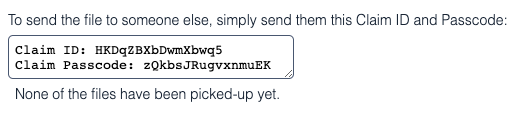
\includegraphics[scale=0.5]{utsend.png}
  \end{center}
   
  \item \textbf{Run the program:} In Pycharm, open the file \texttt{main.py} and run it by right clicking -$>$ `` Run file in Python Console". There should be a pop up window that looks similar as the one below: 
  
  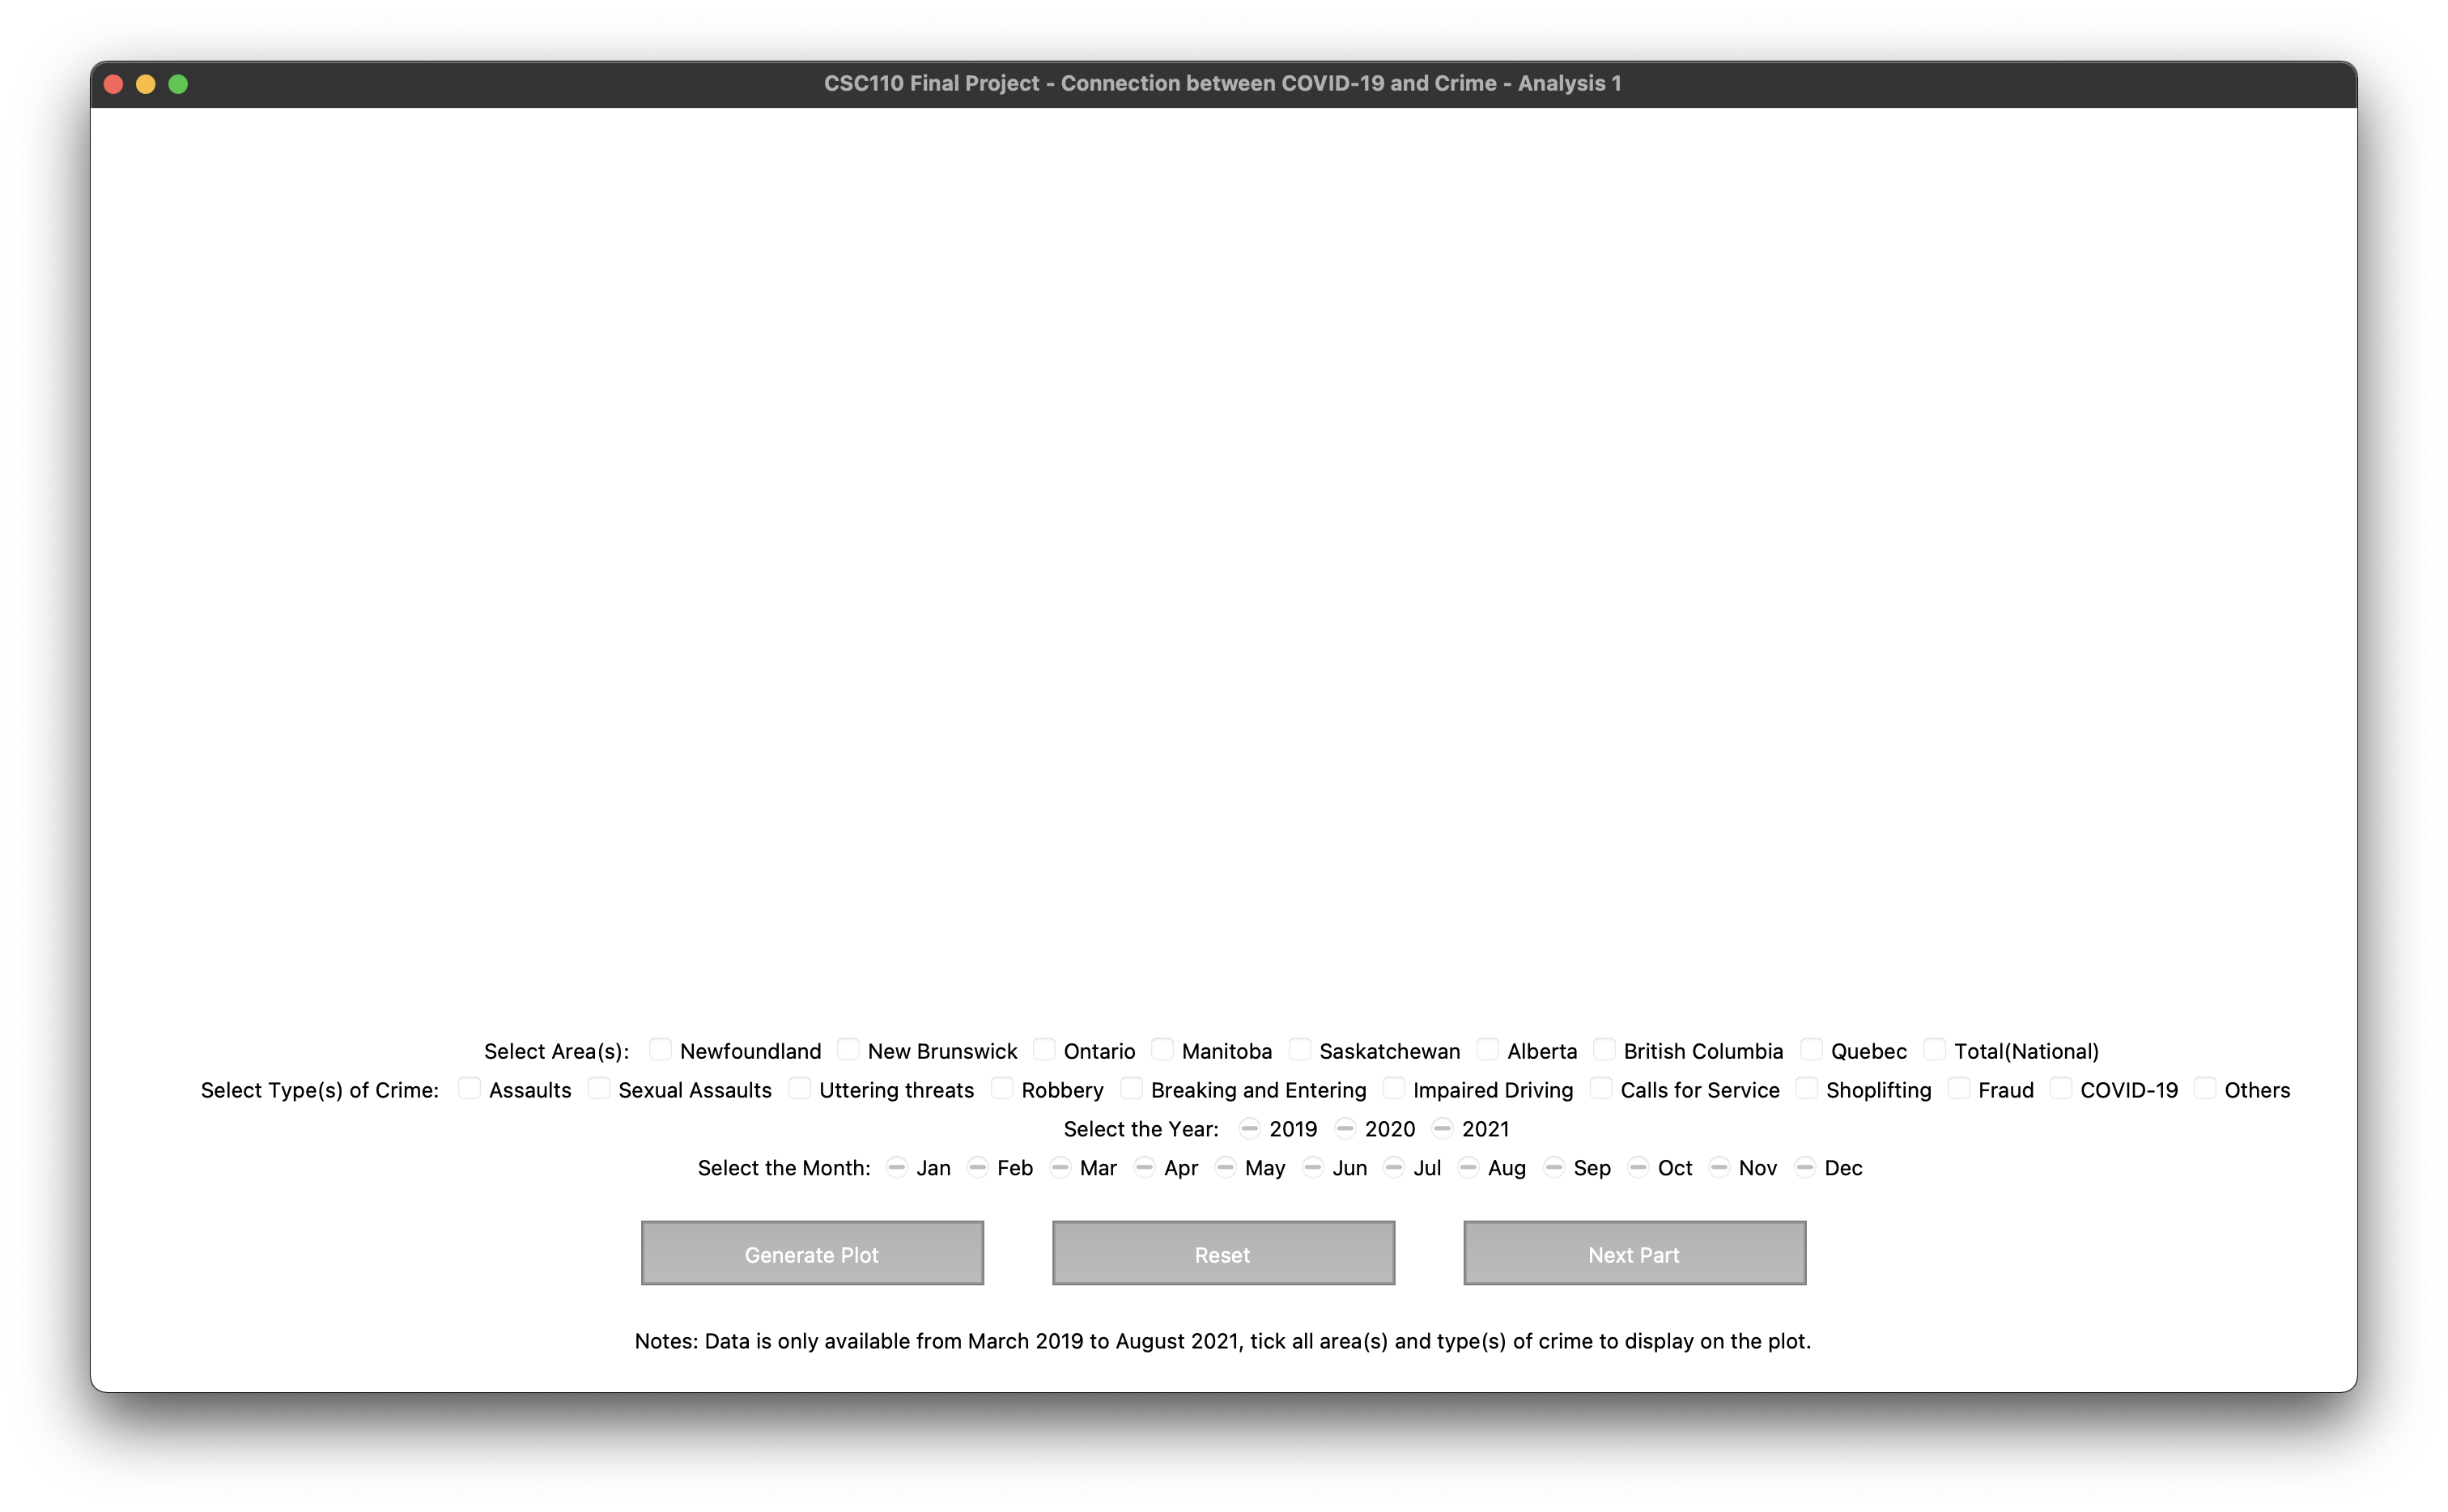
\includegraphics[scale=0.3]{screenshot1.png} 
  
  \item \textbf{Instructions for Analysis 1:} The above window is the graphical user interface for analysis 1. It is able to generate a stacked bar plot of the number of crime case by area and type (of a specific month). To plot a graph, select as many areas and types of crime as you want, select year and month, and click on ``Generate Plot". The program will not plot anything if year or month is not selected, an empty plot is given when none of the area and type is selected. Valid input will plot a graph in the window similar to the two examples below. The font and graph size are adjusted for the best display on a typical lab-top screen, large monitors may cause them to be too small. However, the graph is resizable by adjusting the size of the window.
  
  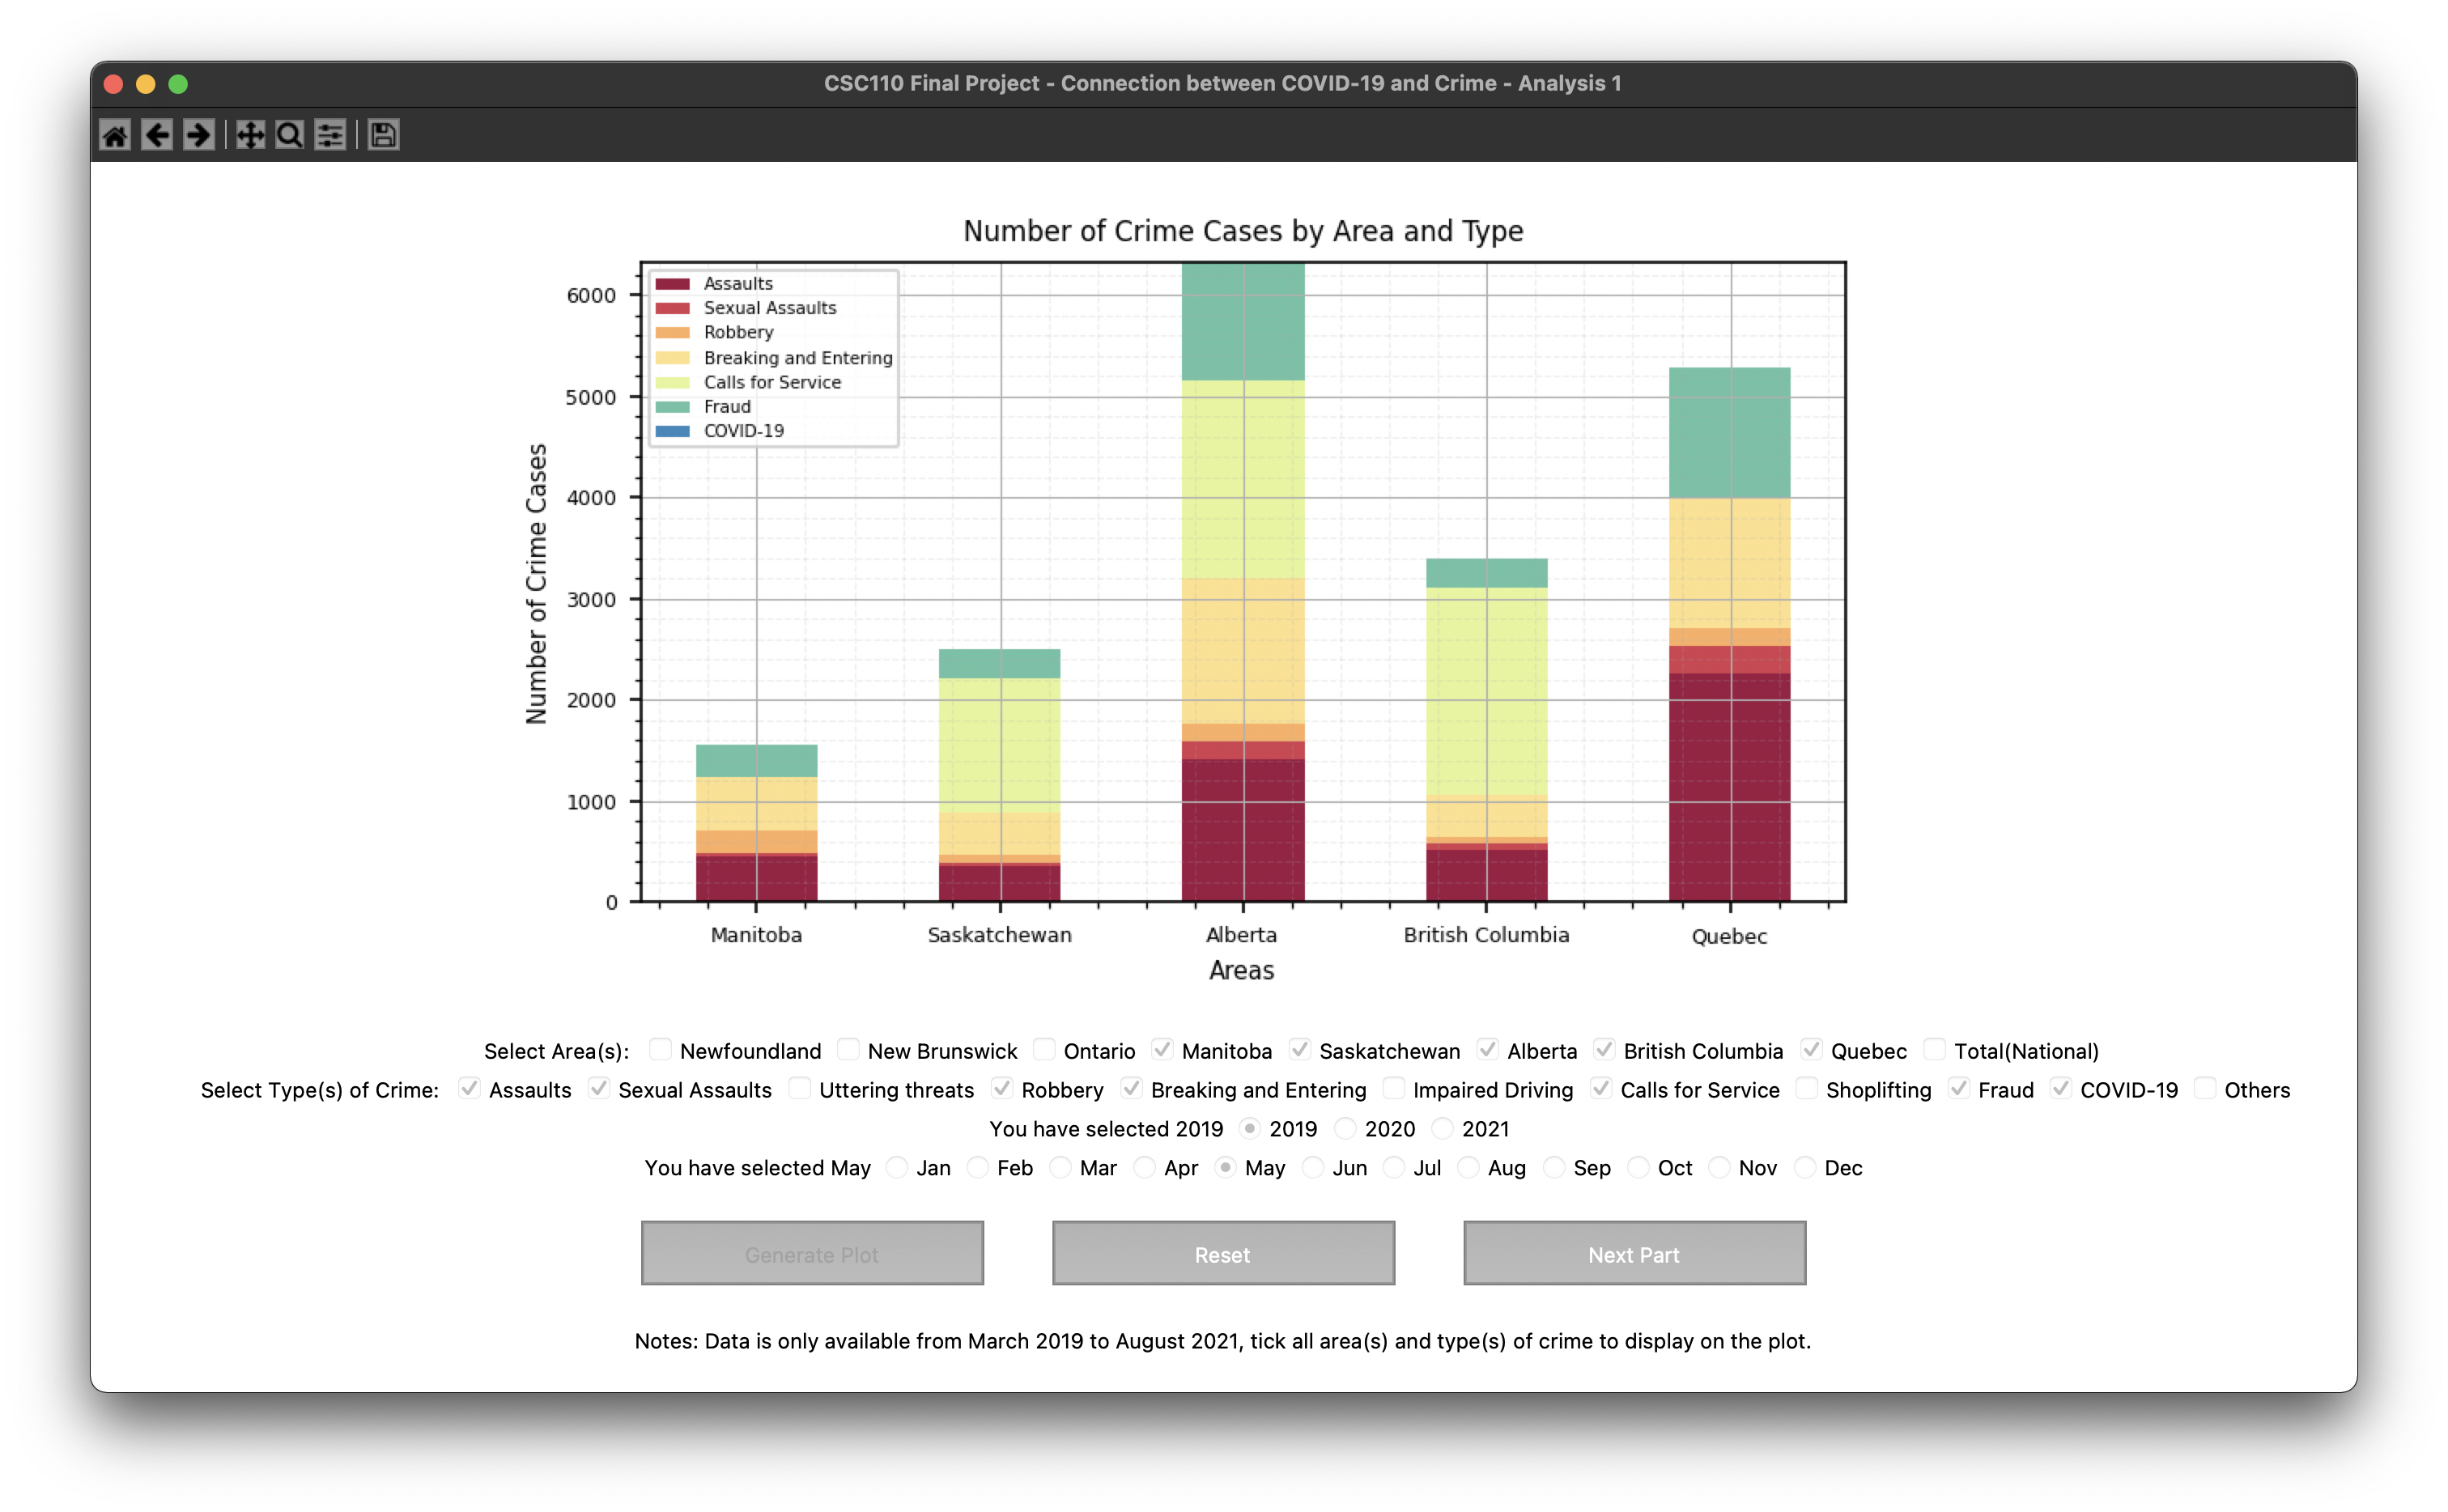
\includegraphics[scale=0.15]{screenshot2.png} 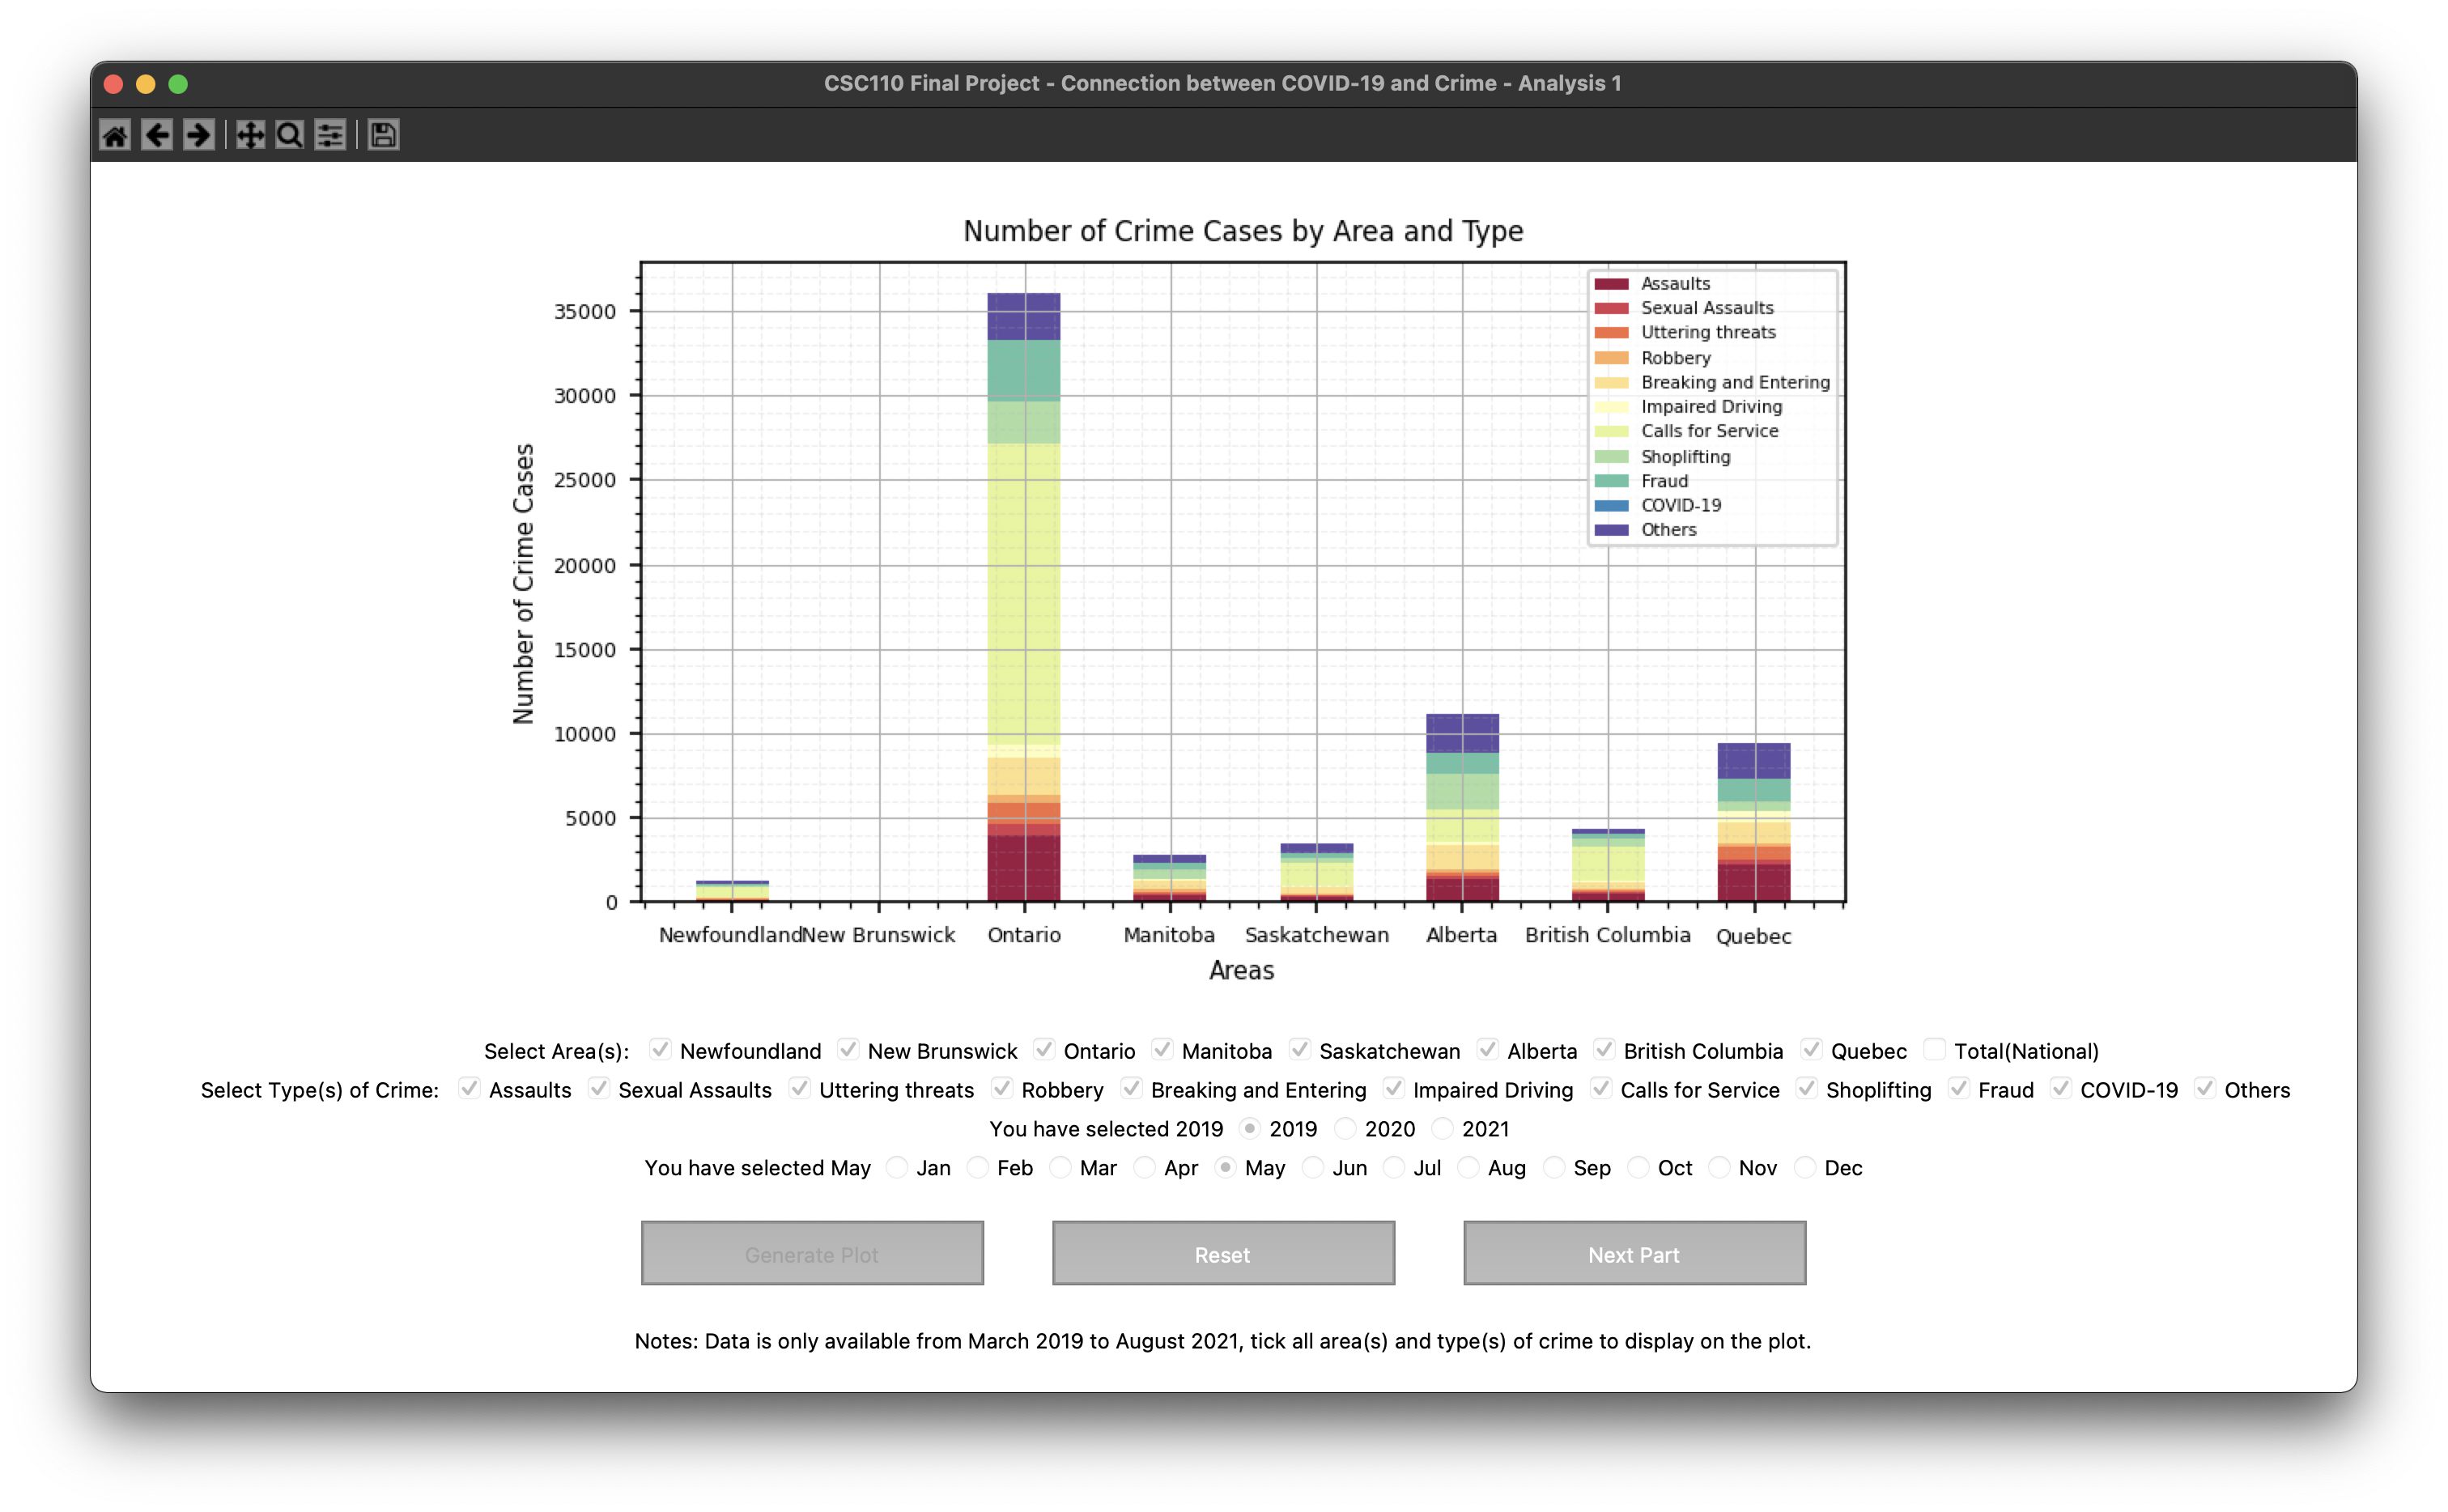
\includegraphics[scale=0.15]{screenshot3.png} 
  
  For each plot, the x-axis is the area you selected, the y-axis is the number of crime cases in the specific year and month. Each color represents one type of crime, as given in the legend (the position of the legend may be different among graphs as it automatically finds the best place to fit in). Note that the graphs are different based on different user inputs. The height of the y-axis also ajust automatically based on the height of the plotted bars. As given in the note at the bottom, data is only available from March 2019 to August 2021, selecting the year and month without data (for example: September 2021) will also result in an empty graph.
  \\
  \\
  Each time a graph is plotted, click on ``Reset" to reset the window, which will result in the exact same window as step 3. The ``Generate Plot" button is disabled until reset button is clicked. Click on ``Next Part" to close the current window and move to the next analysis of our project.
  
  \item \textbf{Instruction for Analysis 2:} A new window should pop out that looks similar to the picture below: 
  
  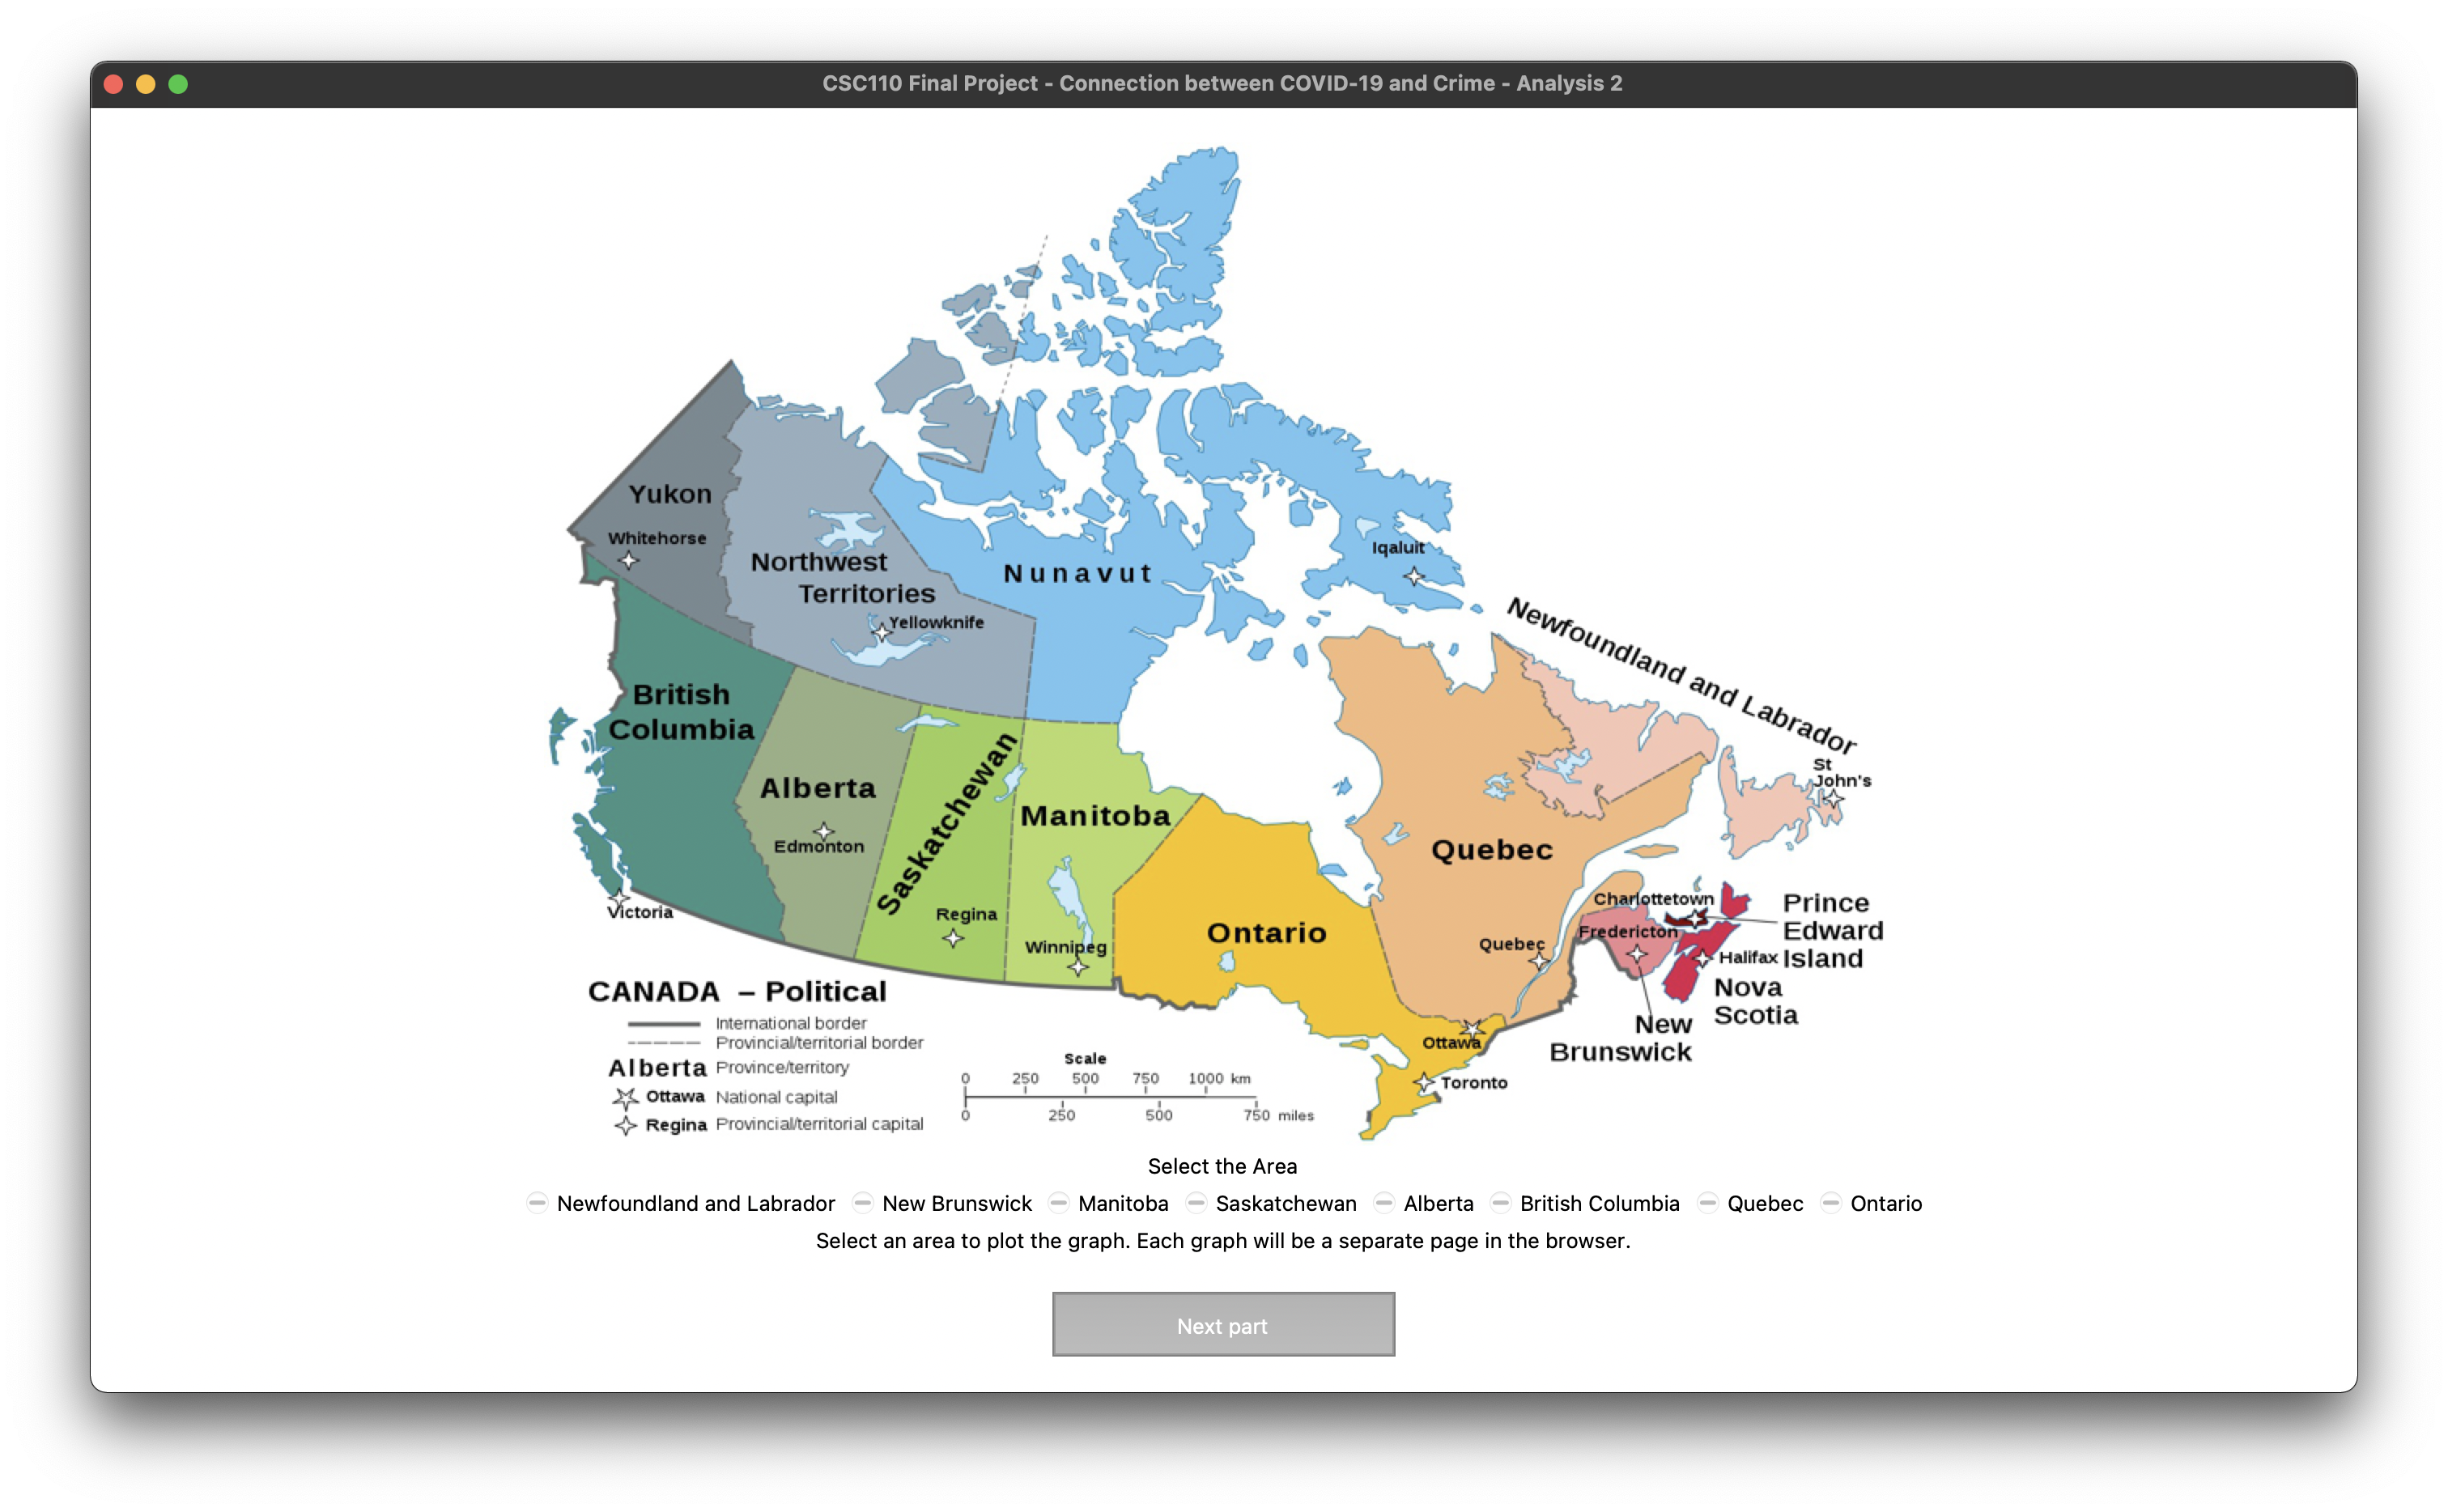
\includegraphics[scale=0.3]{screenshot4.png} 
  
  This analysis will generate line charts that compare the trend of daily crime cases(by type) and daily COVID-19 cases of each province. At the bottom of the window, select an area to generate a plot. Each plot will appear as a separate page in the browser. The current window will not be closed after a plot is generated, you can select another area to create a different plot. Here are two examples of the graphs: 
  
  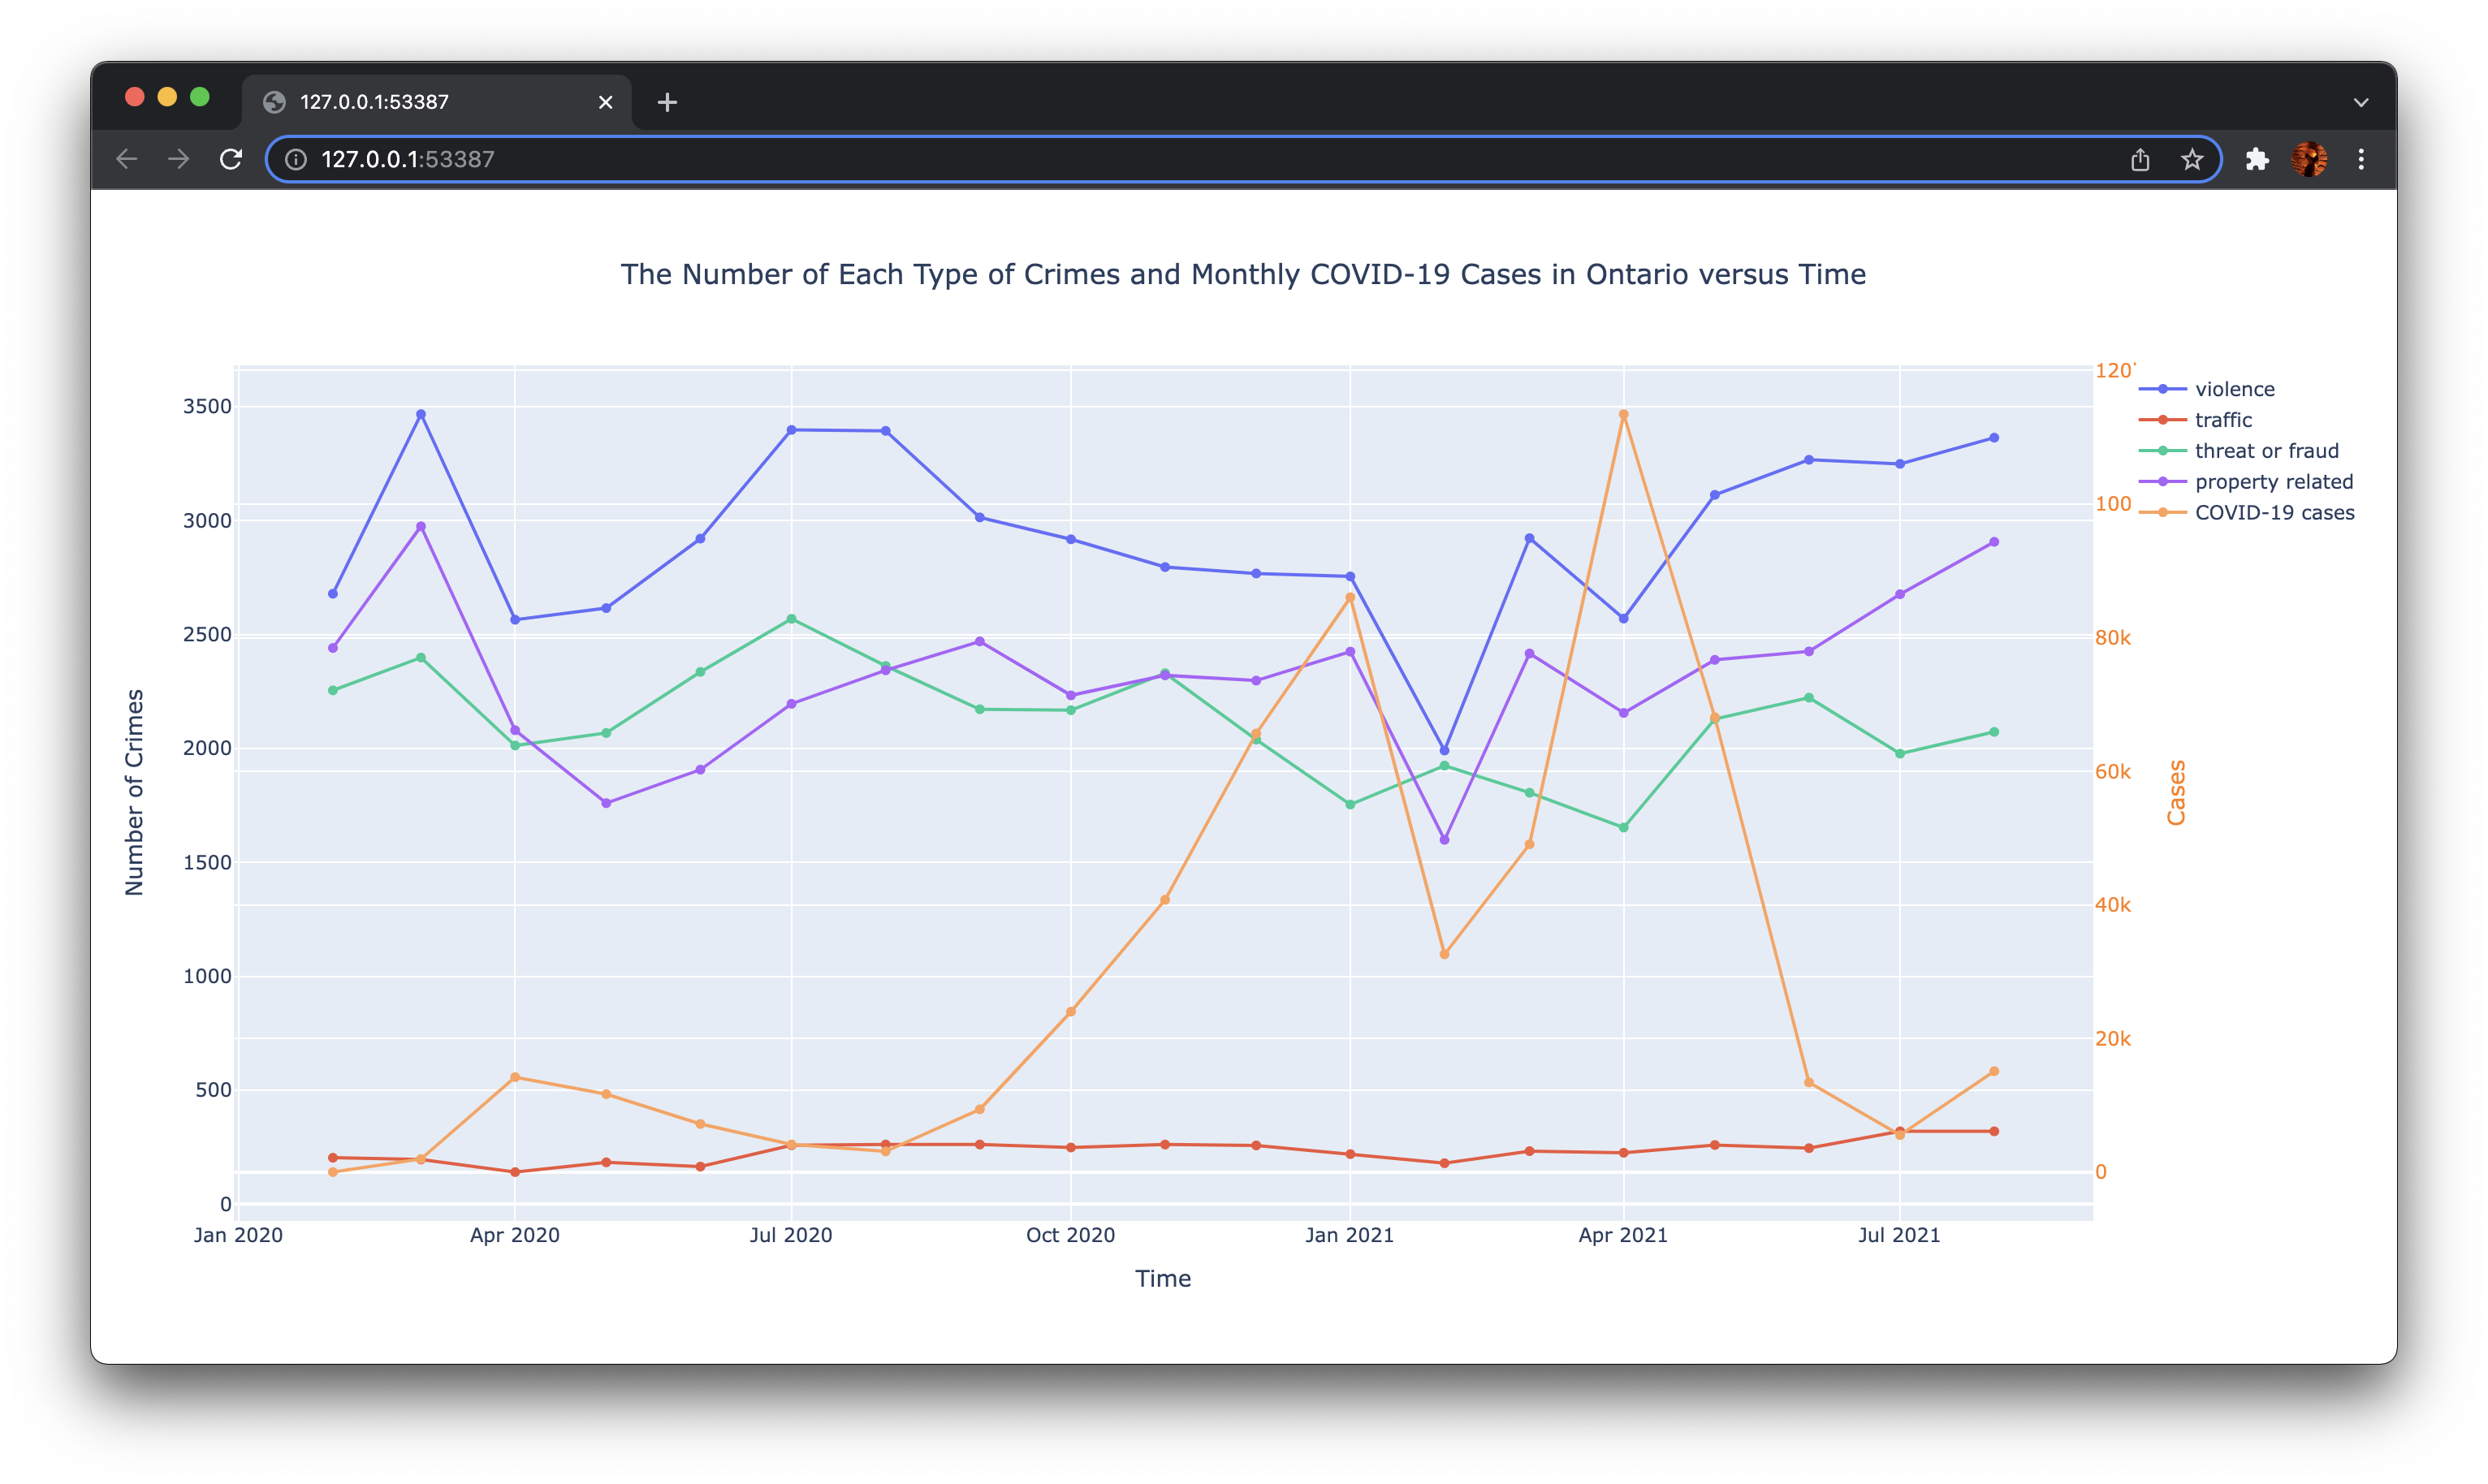
\includegraphics[scale=0.15]{screenshot5.png} 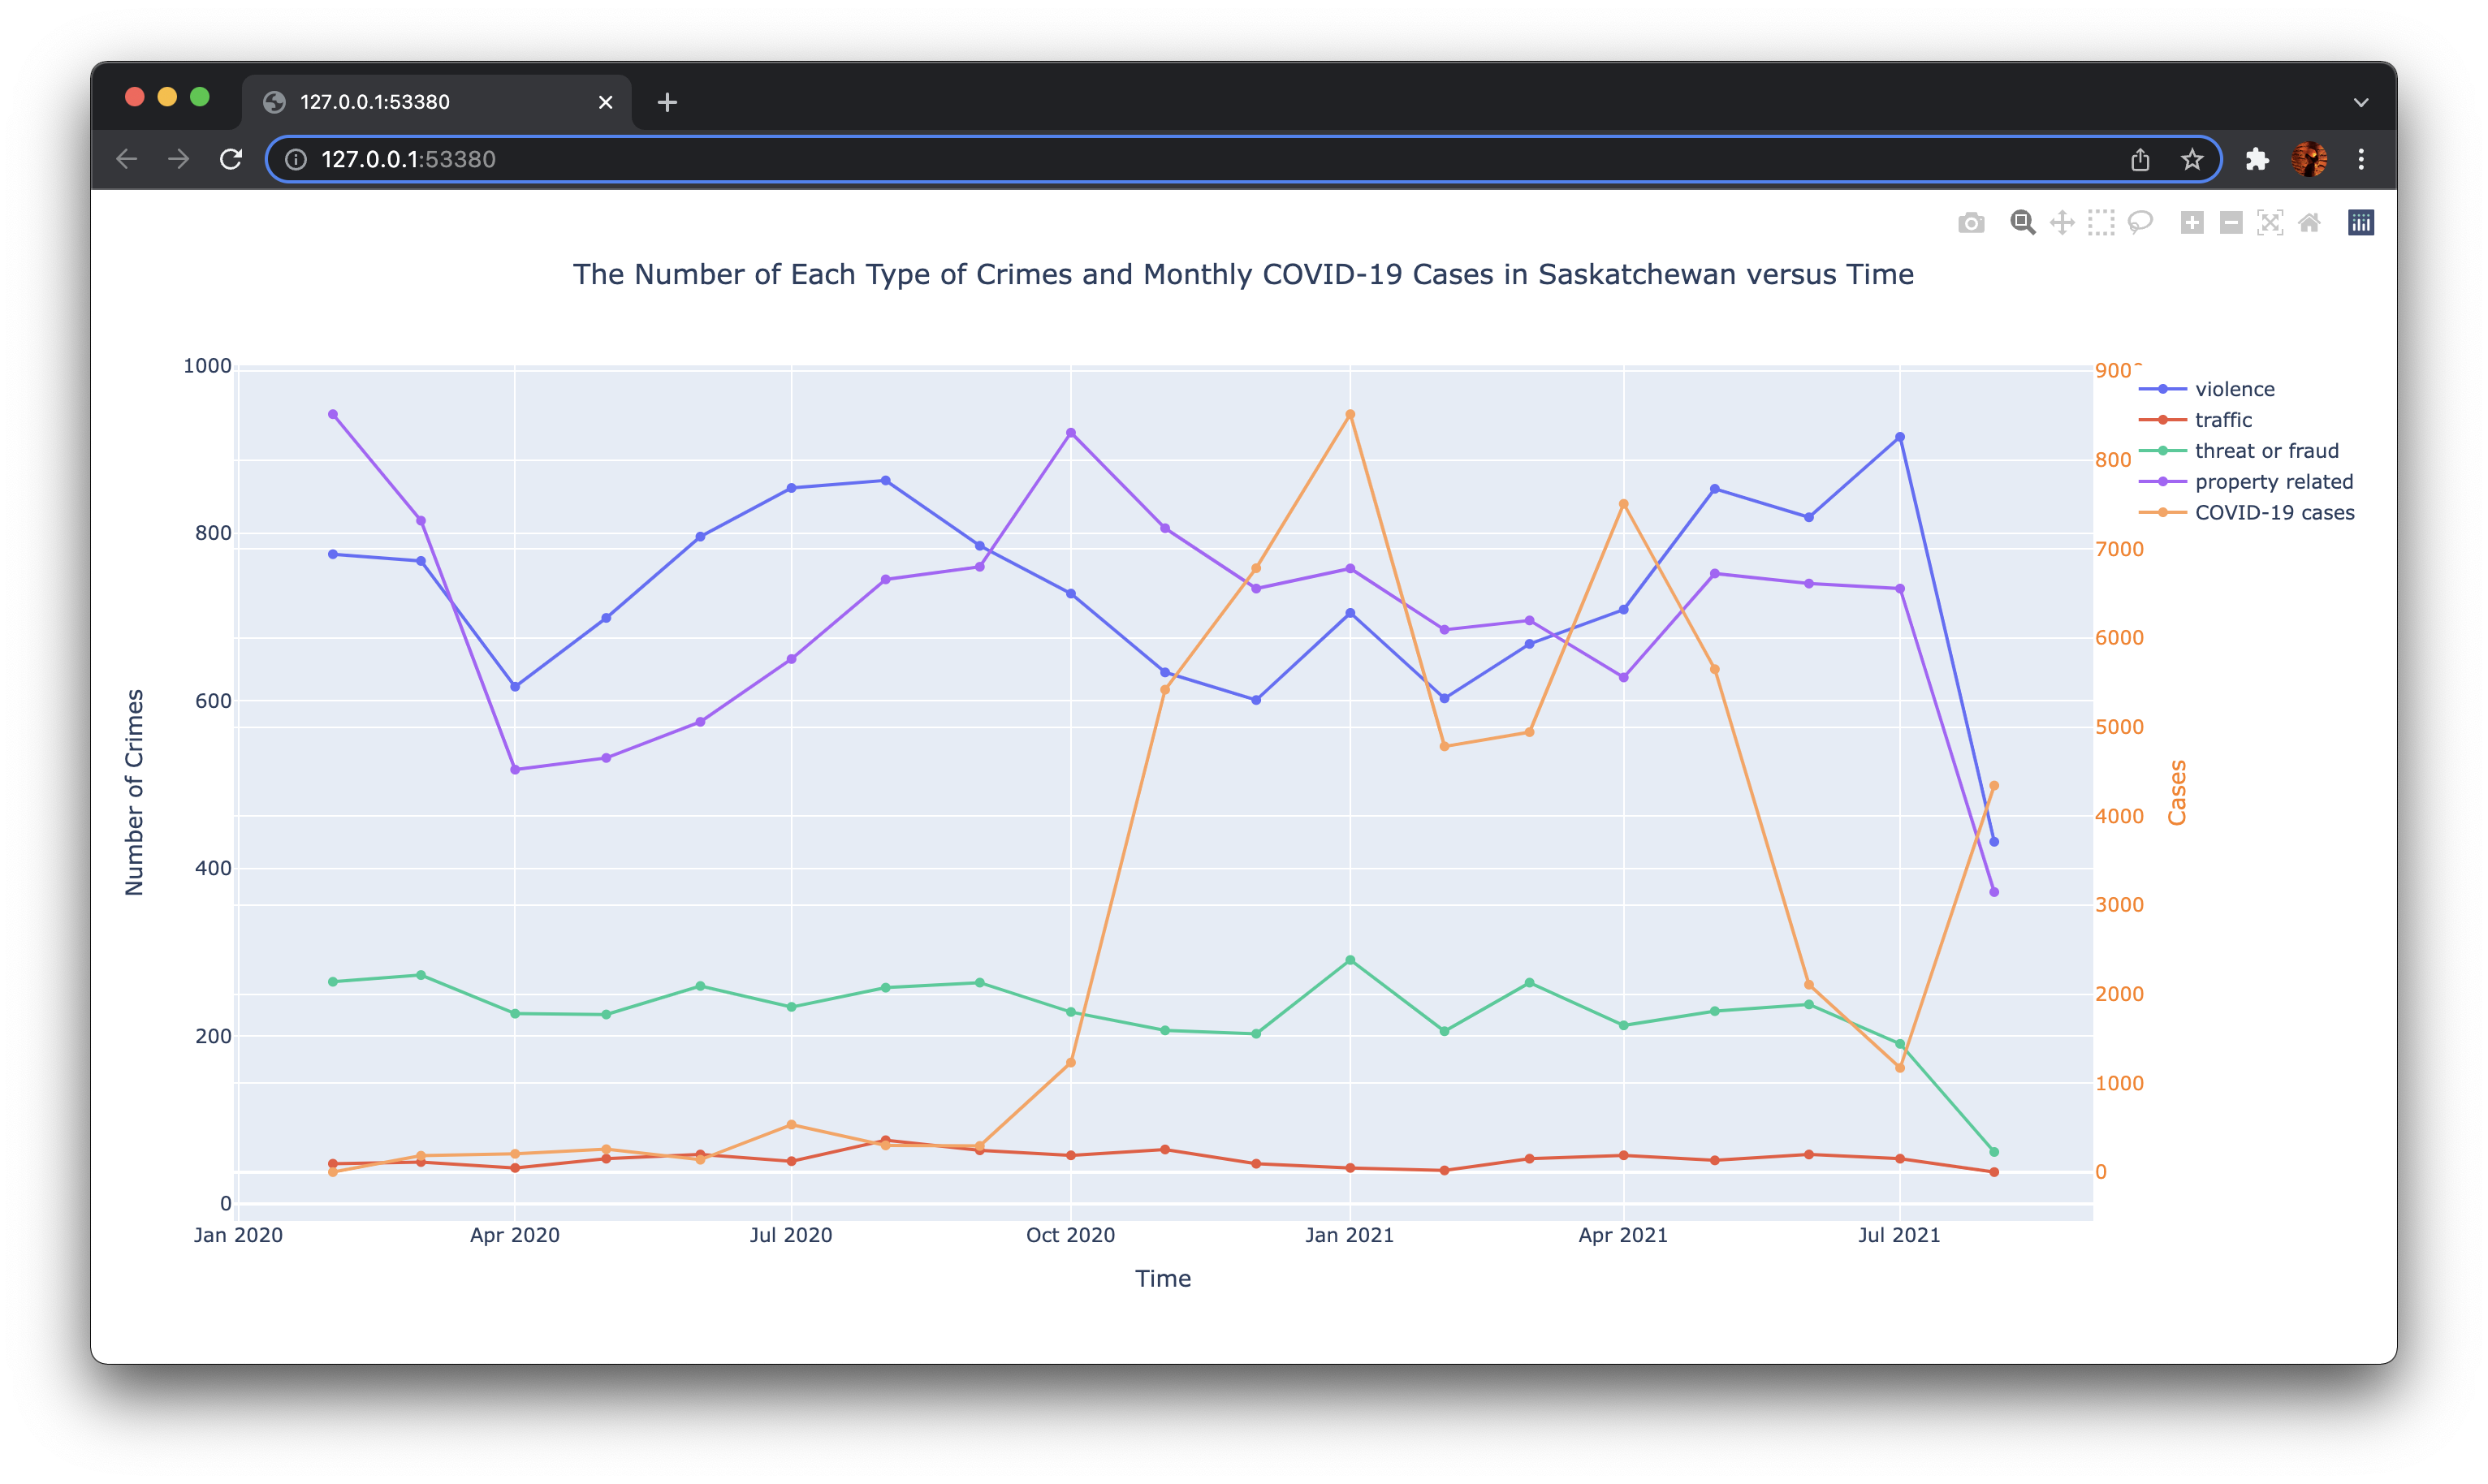
\includegraphics[scale=0.15]{screenshot6.png}
  
  For each plot, the x-axis is time, the left y-axis is the number of crime cases, the right y-axis is the number of COVID-19 cases. Double axes are used since we only care about the trend, not the exact number. The number of COVID-19 cases is significantly higher than crime cases, therefore having just one axis will make it hard to observe the trend of crime cases. 
  \\
  \\
  On the right side of each graph, the legend shows the data that each line corresponds to. Click on one of the color will hide or display that line, double clicking will hide all other lines and display only that line. The user is able to zoom in a specific section of the graph by highlighting the desired area, and go back to the original plot by clicking ``Autoscale" (8th icon in the tool bar on the top right). Click on ``Next Part" to close the current window and move to the next part.
  
  \item \textbf{Instruction for Analysis 3:} A new window should pop out that looks similar to the picture below: 
  
  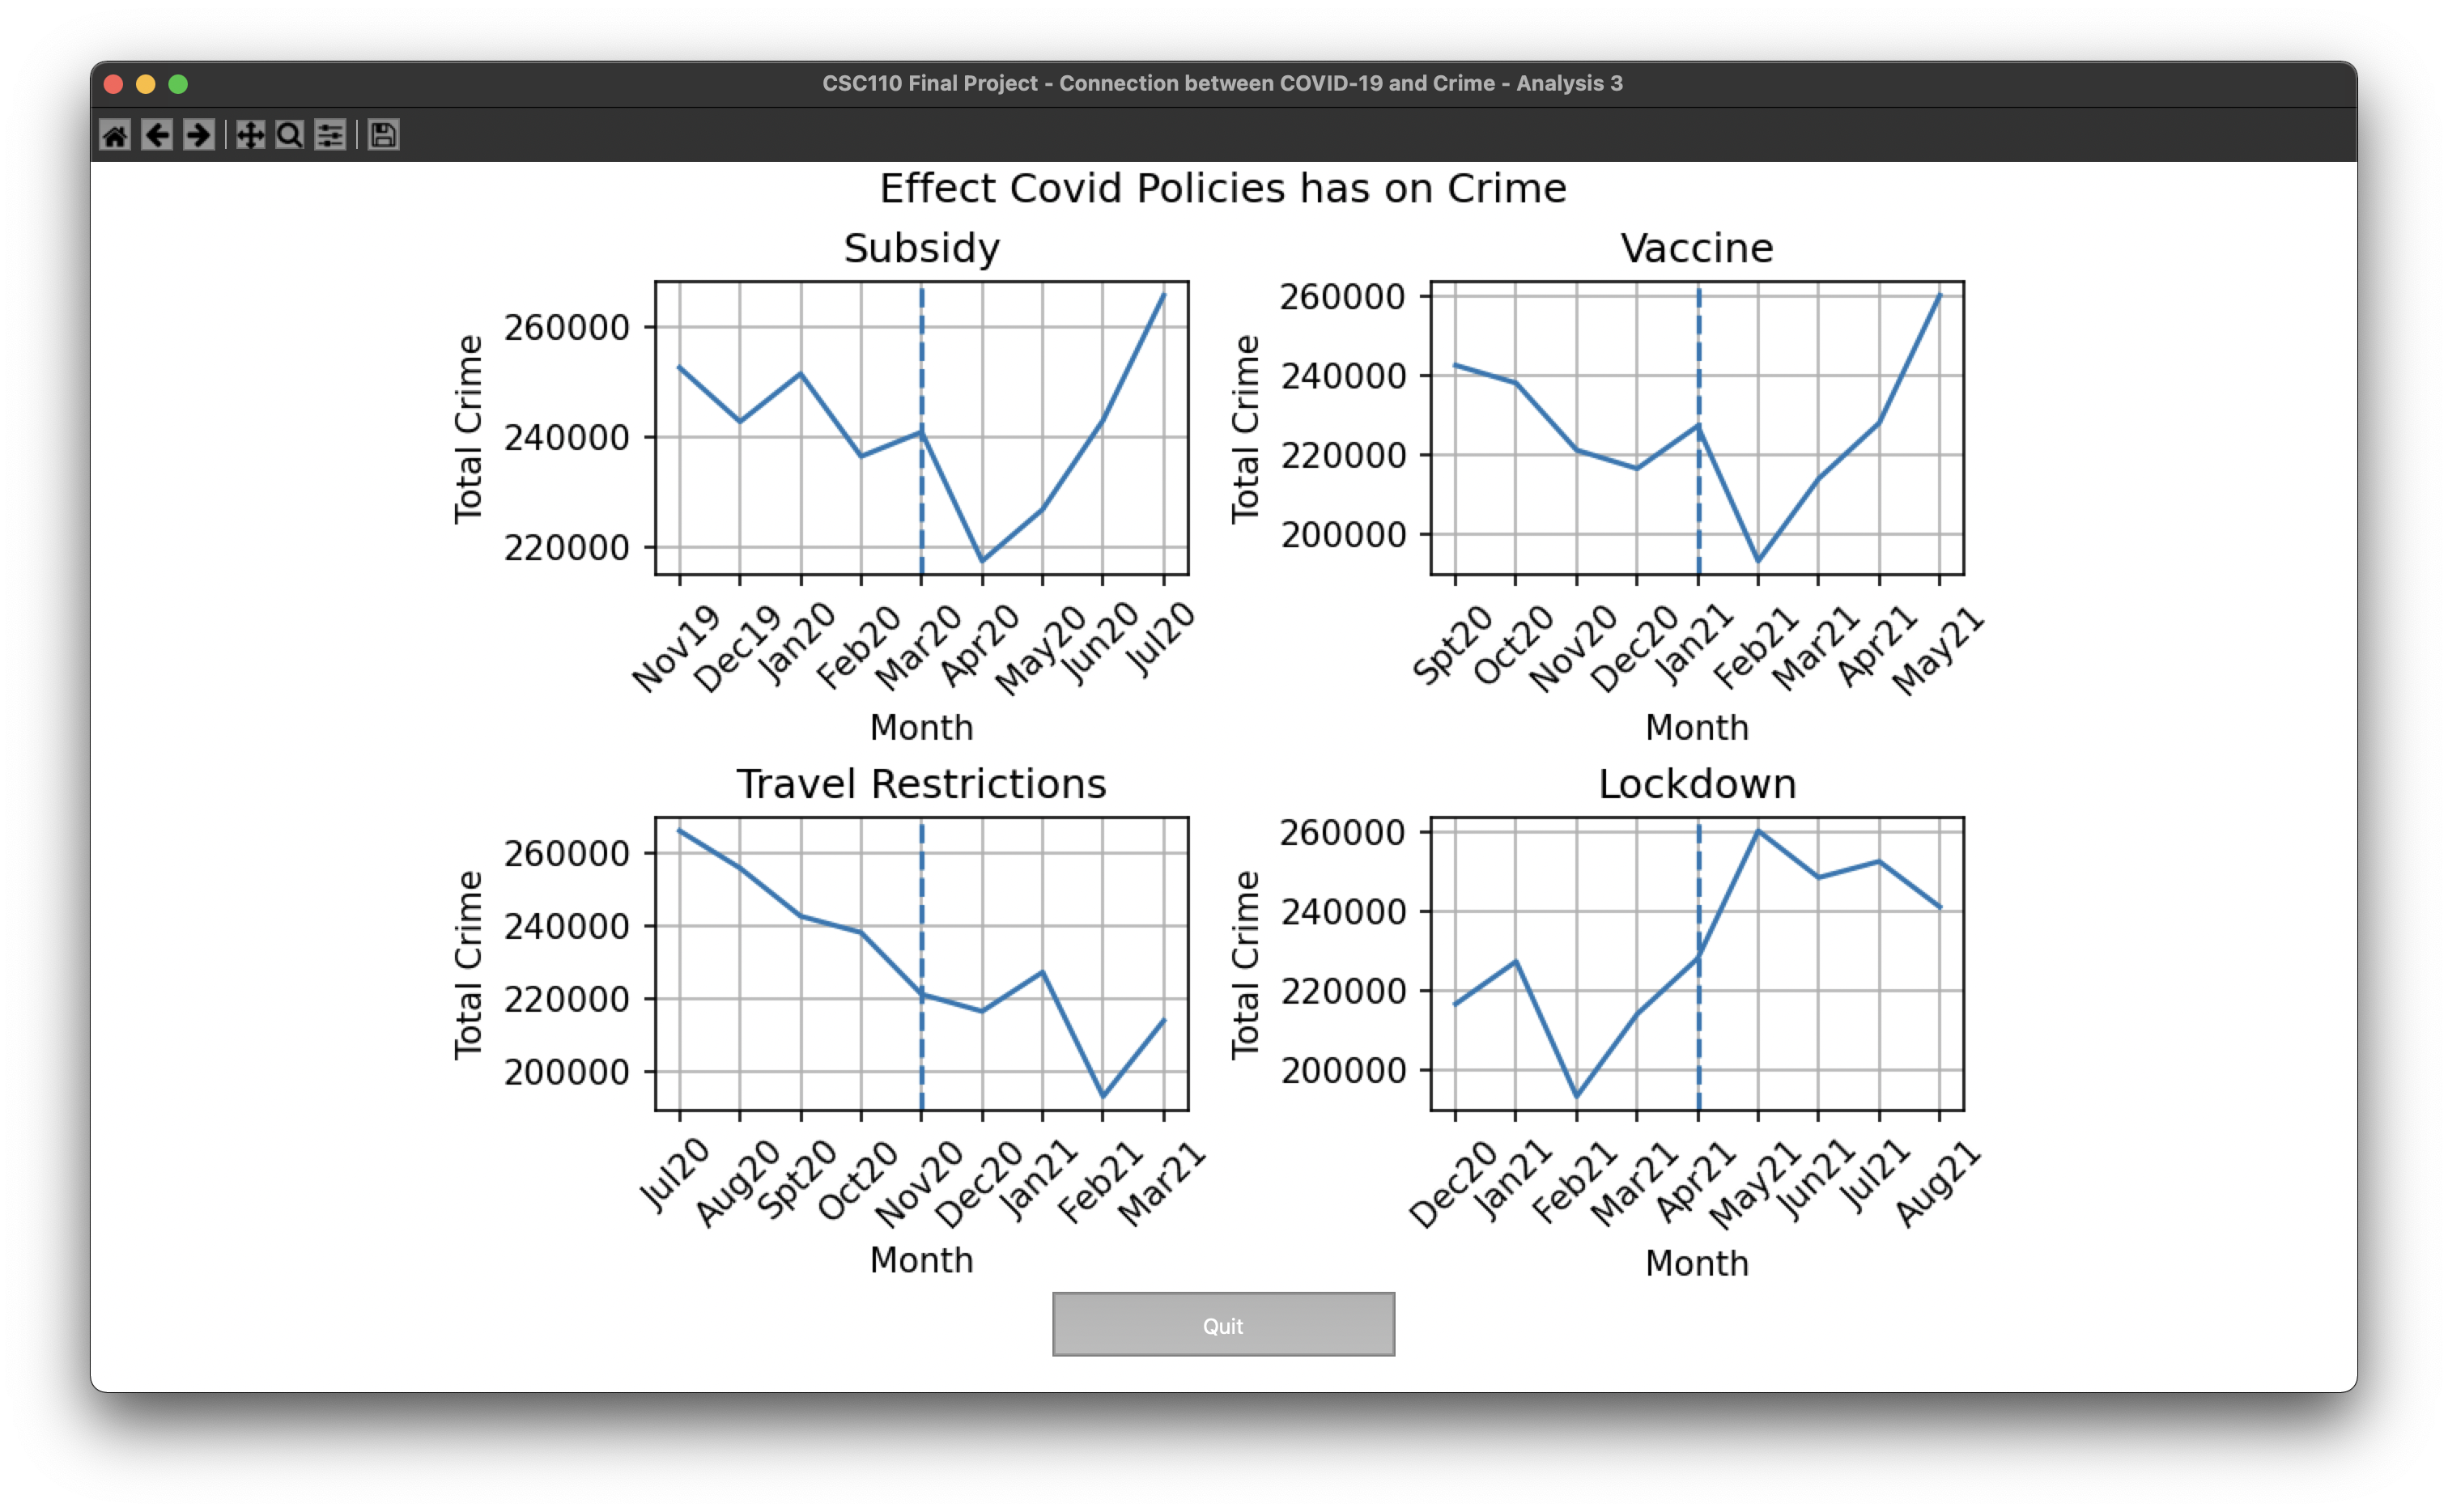
\includegraphics[scale=0.3]{screenshot7.png}
  
  This analysis of our project isn't interactive. It shows the effect of four major COVID-19 related policies on the number of crime cases. Each of the four graph has a doted line in the middle, which represents the date of which the policy was enacted. We compared the difference between the left and right side of the each graph to conclude on the influence that these policies had on crime. Click on ``Quit" to close the window and exit the program.
 
\end{enumerate}

\section*{Changes to Proposal}

As our group worked, our final project ended up straying away from the path of proposed ideas we had originally. The major change was that our proposed idea was to have 4 separate analyses. However, our second and third analysis ended up being too similar and so we decided to combine the two to create an interactive map. This became our second analysis; one that focused mainly on comparing various types of crime with the amount of COVID cases on a provincial level. Our user is able to see a visual representation of all provinces and territories within Canada, where they are then able to select a province or territory to view the corresponding graph of the data. We found that this analysis is more user-friendly than our original ideas, as the interactive maps serves as a method of keeping our data and graphs organized. This ultimately prevents the user from getting overloaded with information. 
\\
\\
Another major change can be found in our first analysis, where we originally planned on creating an animated stacked bar plot. However, we found that we did not have enough data to create an effective animated bar plot as we had enough data for under 30 frames. This resulted in a 1-2 second animation and made the analysis feel both ineffective and incomplete. As a result, we created the GUI, where users are able to select more than one province and crime type, and compare the crime occurrences for the chosen year and month through a stacked bar plot. This GUI worked beautifully, it was both aesthetically pleasing and extremely effective at comparing occurrences of crime types within different provinces. 


\section*{Discussion}
\begin{enumerate}
\item In the first part of our research, Tkinter is used to construct a graphical user interface to visualize the number of different types of crime committed in most Canadian providences within the range of months from March 2019 to August 2021. When comparing the number of robbery cases in April 2019 and 12 months later, April 2020, there is a remarkable difference between the two data sets. For example, the number has dropped from 183 cases to 73 cases in Quebec. Similarly, cases also dropped significantly in Alberta and Manitoba, from 196 to 112 in Manitoba and from 187 to 115 in Alberta. However, there are some exceptions in some of the provinces. In Saskatchewan, the number increased from 35 to 48. Next, when comparing the number of assault cases, it dropped in a range of 22\% and 32\% in the majority of provinces. Although, there is a special case that, in British Columbia, the number increased a little bit (from 450 to 465). 

\item The second part contains eight graphs corresponding to eight provinces with both crime and COVID data. These graphs give a more direct visualization of the relationship between the two data sets from the starting of COVID. There is a notable decrease in all types of crime in almost all graphs around March - April 2019, which is when the number of COVID cases started to rise in Canada. However, the number bounced back right after. Surprisingly, the traffic-related calls were about the same throughout the two-year interval. Our group expected to see a dramatic decrease in this type of crime. We thought COVID made most of the population stayed at home. However, the restrictions did not decrease the occurrence of traffic accidents. One possible answer we came to up to this question is that people adapted more lousy driving habits due to stress or other factors during the pandemic, which caused the drivers to be more likely to speed or drive under the influence. 


\item From our third analysis we were able to graph total crime against time for four major policies that were related to COVID. 
\begin{enumerate}
    \item The first policy we analyzed was the CRB benefit that was introduced at the start of the pandemic in March 2020. This benefit was put into place to provide financial aid for struggling Canadians that have lost work due to COVID. Through our visual representation of the crime rates during the interval centered on this month, we can see a drastic decrease in time for the month after this policy was introduced. This could be directly correlated with the CRB, as the CRB decreased a lot of financial distress among families which in turn reduced the need to commit crimes such as theft and assault. However, figure 1 also shows that shortly after the implementation of the CRB, crime rates reached an all time high peaking at around 270 000 cases. A possibility of this is that many families who received this large sum of "free" government money were financially irresponsibly which ultimately placed them back into a situation of financial distress, which can in turn increase crime rates.

\item From the Vaccine Figure, we can see that there was also a drastic decrease in crime rates for a month, since the date that Canada acquired an additional 20 million vaccine doses. However, in a trend that resembles that of the Subsidy figure, we can see that crime rates have also hit an all time high at around 270 000 cases shortly after reaching an all time low. Our group believes that the first dip in crime is a result of the false sense of security that the vaccine brought with it, and the dramatic climb in crime shortly after is caused by the realization of the risks associated with the vaccine, as more and more vaccine related problems were reported by the media. 
\item In our third figure, we analyzed the effect travel restrictions have had on crime. As there have been many different travel restrictions, we chose the travel restriction that was implemented in November 2020, when the government announced that non-essential travel would be restricted until the end of January. Taking a look at the trend line here, we can see that the general trend from July 2020 to January 2020 is decreasing, as this is the period where non-essential travel was still limited. We attributed the decrease in crime to the decrease in people coming into the country due to the travel restrictions. AS we can see, when the travel restriction was removed in February - March, the crime count started to climb again. 

\item For our final figure, we took a look at the effect the Lockdown has had on crime. To prevent any big time overlaps with out other figures, we chose to analyze the recent lockdown in April 2021. This analysis is a bit interesting as one might predict a decrease in crime as a result of lock downs. However, the opposite happens here as we have a growth in the crime count after the lockdown was put into place. Considering that this was not the first lockdown, and that there was a large amount of individuals dissatisfied with the government policies and constant lock downs; we believed that this public dissatisfaction was the root cause of the increase in crime during the second half of this interval.
\end{enumerate}

\item The most significant limitation we faced during the project is that our crime data set does not have data for all provinces. Even though we already have a big data set of all crime records in Canada for the past two years, the crime data set does not contain data for Prince Edward Island, Nova Scotia, Northwest Territories, Nunavut and Yukon. We also encountered a couple problems with Tkinter, as it was difficult to connect all three analyses together through interactive buttons. Overall, the project's result were also somehow different from our expectations before starting. We thought COVID, government policies, and restrictions would significantly impact the number of different types of criminal cases in Canada. However,some of the results were unexpected such as financial aid causing a rise in crime, or a lockdown resulting in an increase in crime as well, Overall, major COVID policies still had an impact on the crime rates; for the better or for the worse. 

\item If possible, the next step we will take is to investigate the different types of COVID(covid variants) and see if there is a relation between crime as new COVID types are being discovered, then we can also write an algorithm that is able to use past crime data and trends to make predictions based on the amount of future COVID cases and crime occurrences. As our data is fixed, we are also interested in investigating a way where we could filter live data to make computations to display more updated and accurate data. As a next step, our group also plans on dealing with larger data sets as we expand our program on a national scale. \end{enumerate}

\section*{References}

Canadian Institute for Health Information, C. I. of H. I. (2021, October 7). \emph{Covid-19 intervention timeline in Canada.}

\qquad COVID-19 Intervention Timeline in Canada. Retrieved November 5, 2021, from https://www.cihi.ca/en/covid

\qquad -19-intervention-timeline-in-canada.
\\\\Government of Canada, S. C. (2021, April 14). \emph{Selected police-reported crime and calls for service during the}

\qquad\emph{COVID-19 pandemic, March to October 2020}. The Daily. Retrieved November 5, 2021, 

\qquad from https://www150.statcan.gc.ca/n1/daily-quotidien/210127/dq210127c-eng.htm.
\\\\Government of Canada, S. C. (2021, November 4). \emph{Selected police-reported crime and calls for service during}

\qquad \emph{the COVID-19 pandemic.} Retrieved November 5, 2021, from 

\qquad https://www150.statcan.gc.ca/t1/tbl1/en/tv.action?pid=3510016901\&pickMembers\%5B0\%5D=1.20\&

\qquad cubeTimeFrame.startMonth=01\&cubeTimeFrame.startYear=2019\&cubeTimeFrame.endMonth=12

\qquad \&cubeTimeFrame.endYear\=2021\&referencePeriods\=20190101\%2C20211201. 
\\\\Public Health Agency of Canada, S. C. (2021, May 28). \emph{Covid-19 Daily Epidemiology update.} Canada.ca. 

\qquad Retrieved November 5, 2021, from https://health-infobase.canada.ca/covid-19/epidemiological

\qquad -summary-covid-19-cases.html. 
\\\\“Timeline: A Year of Pandemic Life in Toronto.” CityNews, https://toronto.citynews.ca/2021/03/11/timeline

\qquad -a-year-of-pandemic-life/. 
\\\\Canada, Department of Finance. “Government Introduces Canada Emergency Response Benefit to Help 

\quadd Workers and Businesses.” Canada.ca, Government of Canada, 2 Apr. 2020, https://www.canada.ca/en/department

\quadd -finance/news/2020/03/introduces-canada-emergency-response-benefit-to-help-workers-and-businesses.html. 
\\\\“Ontario Extends COVID-19 Stay-at-Home Order to May 20, Tightens Restrictions, and Increases Workplace

\quadd Inspections.” The National Law Review, https://www.natlawreview.com/article/ontario-extends-

\quadd covid-19-stay-home-order-to-may-20-tightens-restrictions-and. 
\\\\ Canada, Public Safety. “Government Extends International Travel Restrictions.” Canada.ca, Government

\quadd of Canada, 30 Oct. 2020, https://www.canada.ca/en/public-safety-canada/news/2020/10/government

\quadd -extends-international-travel-restrictions.html. 


% NOTE: LaTeX does have a built-in way of generating references automatically,
% but it's a bit tricky to use so we STRONGLY recommend writing your references
% manually, using a standard academic format like APA or MLA.
% (E.g., https://owl.purdue.edu/owl/research_and_citation/apa_style/apa_formatting_and_style_guide/general_format.html) z

\end{document}
